\chapter{Model}
\label{cha:model}

This chapter covers the details about the two models previously introduced in Chapter \ref{cha:introduction}, where a high level introduction to both the \firstmodel{} and the \secondmodel{} was given.
It follows a top down approach.
General concepts from both types of model are outlined first and the specific details from each model are given afterwards.

As a reminder of the previous chapter a very brief definition of the two models follows.
Both models are quite similar, they represent a way to connect words with meanings.
Both meanings and words are given probabilities of being used, from which information theoretic measures are derived, which are ultimately used to obtain a cost function.
The high level differentiating trait is the way in which the probability of a meaning is obtained.
In the first studied model (\firstmodel{}), the probabilities of both words and meanings are proportional to the number of connections.
In the second model (\secondmodel{}), the probabilities of meanings come from a distribution of \emph{a priori} probabilities.

The remainder of this chapter is divided into two sections.
Section \ref{sec:model_math} deals with the mathematical definitions of the models and it is more theoretical in nature.
Section \ref{sec:model_compute} outlines the computational aspects of the two models and it is more practical and implementation oriented.
This chapter does not deal with any actual details of the implementation of the model.
These details can be found in Chapter \ref{cha:methods}.

Note that Chapter \ref{cha:introduction} offers a high level revision of the graph theory and information theory concepts that will appear during the rest of this chapter.

\section{Mathematical aspect}
\label{sec:model_math}

This section covers the mathematical definition of the model.
Section \ref{sec:model_math_graph} introduces concepts common to both models.
These concepts are then extended for either the \firstmodel{} or the \secondmodel{} in Sections \ref{sec:model_math_first-model} and \ref{sec:model_math_second-model} respectively.

\subsection{Common concepts}
\label{sec:model_math_graph}

In this section, mathematical definitions and notation common to both models is given.
They will be used throughout the remainder of the thesis.

Both models studied in this thesis are based on the idea of a bipartite graph $G_{n,m}$.
Bipartite graphs are comprised of two sets of elements and edges can only appear between an element of one set and an element of the other.

Our two sets are $S$ and $R$.
$S$ is a set of size $n$ containing all words.
The notation $s_i$ is used to refer to some element $i$ of the set $S$.
$R$ is a set of size $m$ containing all meanings.
The notation $r_j$ is used to refer to some element $j$ of the set $R$.

The bipartite graph is represented using the adjacency matrix $A_{n,m}$ (or simply $A$) in most cases.
$A_{n,m}$ is a \nbym{} binary matrix representing whether an edge exists or not in the graph.
Mathematically, each element of the matrix $A$ is defined as
\begin{equation*}
  %\label{eq:definition-aij}
  a_{i,j} =
  \begin{cases}
    1 & \text{if there exists an edge between $s_i \in S$ and $r_j \in R$} \\
    0 & \text{otherwise.}
  \end{cases}
\end{equation*}

In some cases it is more convenient to represent the bipartite graph as the set $E$ of all edges,
\begin{equation*}
  %\label{eq:definition-E}
  E = \Set{(s_i,r_j)}{\text{there exists an edge between $s_i \in S$ and $r_j \in R$}}.
\end{equation*}
For brevity, the tuple $(s_i, r_j)$ is sometimes replaced by the simpler form $(i,j)$.

A notation is defined for the degree of the vertices in the graph.
The word $s_i$ has degree $\mu_i$, while the meaning $r_j$ has degree $\omega_j$.
Mathematically, $\mu$ and $\omega$ are defined
\begin{equation}
  \label{eq:definition-mu}
  \mu_i = \sum_{j=1}^m a_{i,j}
\end{equation}
and
\begin{equation}
  \label{eq:definition-omega}
  \omega_j = \sum_{i=1}^n a_{i,j}.
\end{equation}

There is an additional parameter of the models, $\phi$, which is not directly related to the bipartite graph.
This parameter appears in both models and it is used to ``emphasize'' the effect of the vertex degrees in the calculations.
As explained in previous sections, this parameter is a new addition to the models originally presented in \cite{Ferrer2005a} and \cite{Ferrer2003a}.

Figure \ref{fig:graph-example-base} displays an example of a simple $G_{3,3}$ graph.
A graphical representation is included, as well as the corresponding values of the mathematical concepts discussed in this section up to here.

\begin{figure}
  \centering
  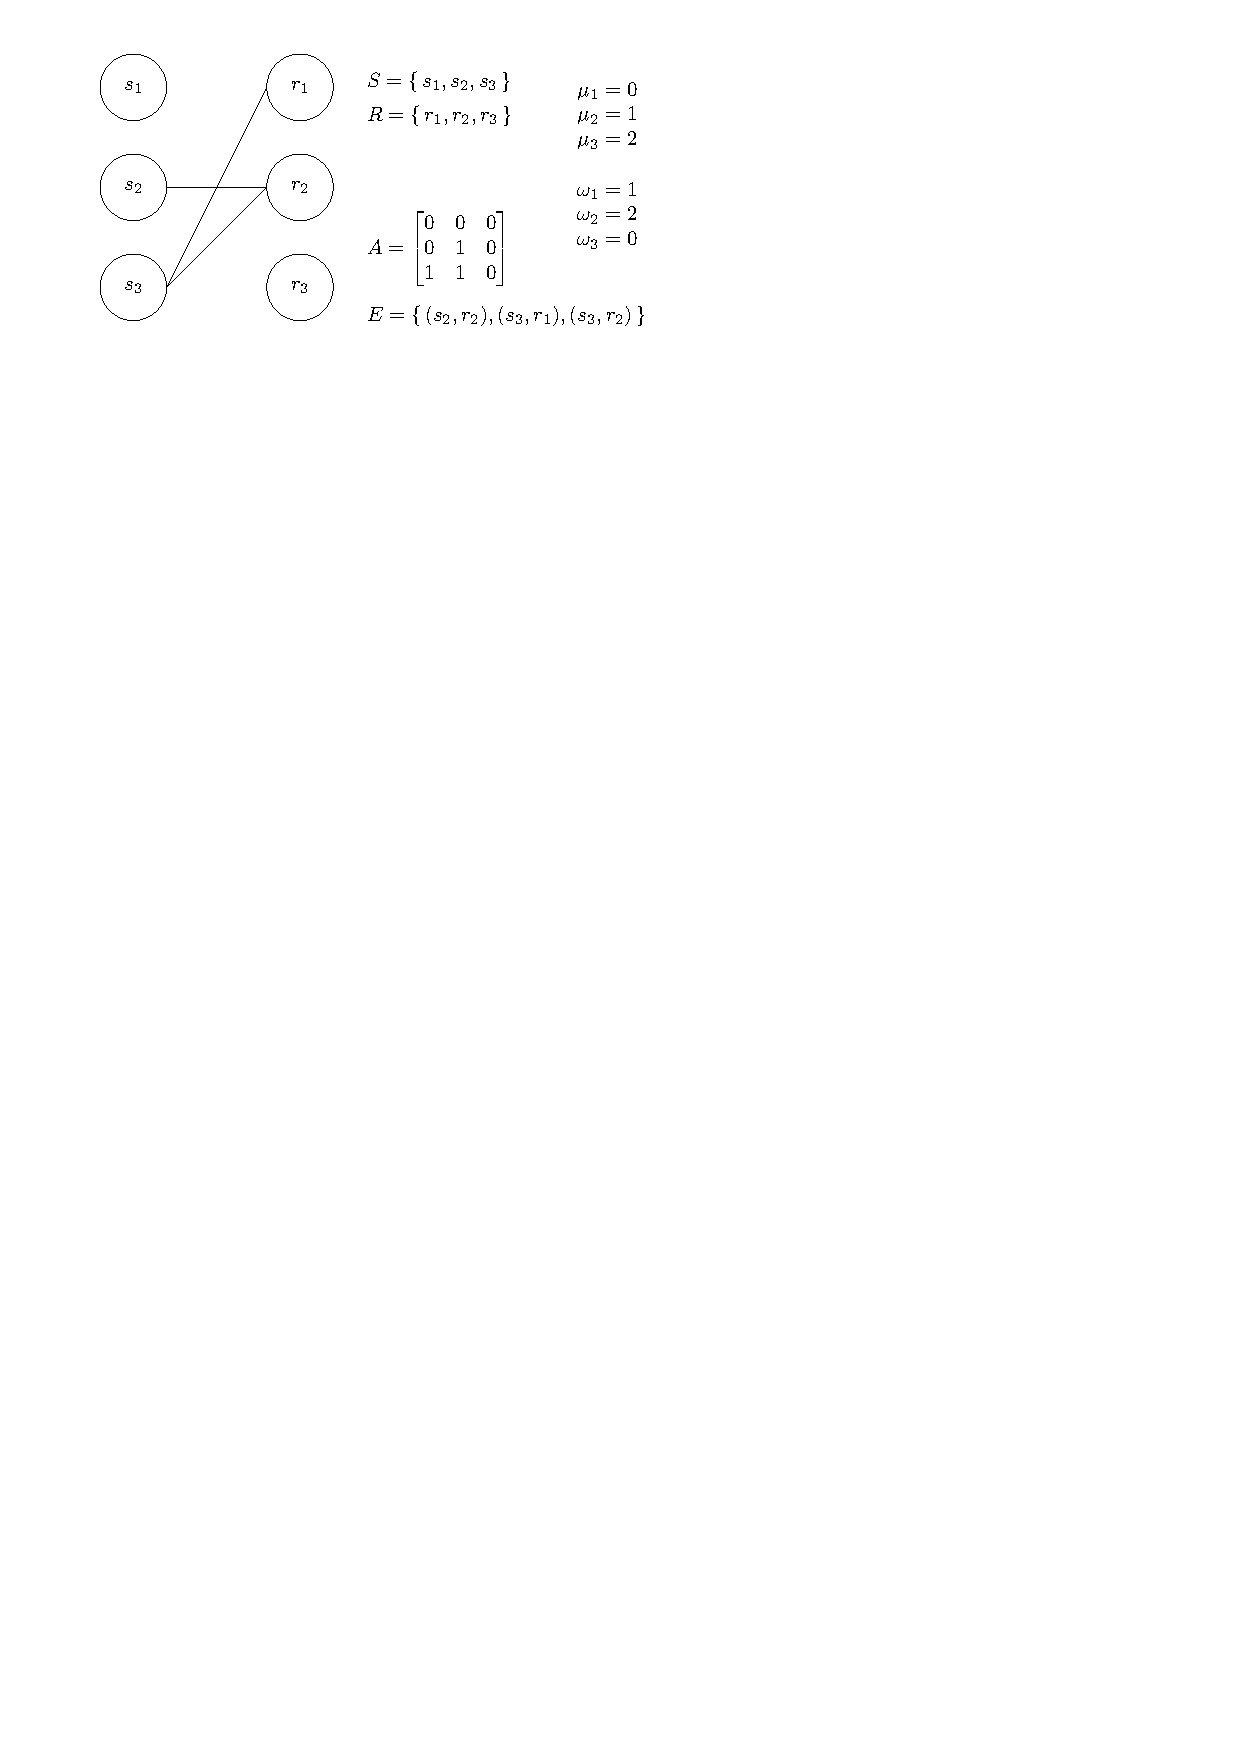
\includegraphics[width=\textwidth]{graph_example_base}
  \caption{%
    A $G_{3,3}$ bipartite graph with the corresponding adjacency matrix $A$, set of edges $E$ and vertex degrees $\mu$ and $\omega$ for each vertex.
  }
  \label{fig:graph-example-base}
\end{figure}

With the parameter $\phi$, the definitions of $\mu$ and $\omega$ can be generalized.
$\mu_\phi$ and $\omega_\phi$ are defined as
\begin{equation}
  \label{eq:definition-muphi}
  \mu_{\phi,i} = \sum_{j=1}^m a_{i,j} \omega_j^\phi
\end{equation}
and
\begin{equation}
  \label{eq:definition-omegaphi}
  \omega_{\phi,i} = \sum_{i=1}^n a_{i,j} \mu_i^\phi.
\end{equation}
It can be seen that when $\phi=0$ Equation \eqref{eq:definition-muphi} becomes Equation \eqref{eq:definition-mu} and Equation \eqref{eq:definition-omegaphi} becomes Equation \eqref{eq:definition-omega}.
In other words, $\mu_{0,i} = \mu_i$ and $\omega_{0,j} = \omega_j$

\subsection{The \firstmodel{}}
\label{sec:model_math_first-model}

This model is defined by the joint probability of a word $s_i$ and a meaning $r_j$.
This probability must be proportional to the product of the degrees of $s_i$ and $r_j$ and it must be zero if there is no edge between $s_i$ and $r_j$.
Mathematically,
\begin{equation*}
  %\label{eq:psirj-proportional-mui-wj}
  p(s_i, r_j) \propto a_{i,j} (\mu_i \omega_j)^\phi,
\end{equation*}
where the parameter $\phi$ is used to control the effect of the vertex degrees.
As previously noted, the original model from \cite{Ferrer2005a} is equivalent to this one but with $\phi=0$ and so, the vertex degrees have no effect in the joint probability. \redtxt{no ho tinc gaire clar... desde on ``comencen'' les equacions del primer model?}

From this definition, equations for the marginal probabilities are derived, which in turn are used to obtain the information theory expressions in the cost function $\Omega$ (Equation \eqref{eq:definition-Omega}).
From these expressions, dynamic equations are derived to obtain the change experienced by the entropies after a single mutation has occurred on the adjacency matrix $A$.

\subsubsection{Joint Probability}

Adding a normalizing factor $M_\phi$, the joint probability becomes
\begin{equation}
  \label{eq:definition-psirj_first-model}
  p(s_i, r_j) = \frac{1}{M_\phi} a_{i,j} (\mu_i \omega_j)^\phi.
\end{equation}

This normalizing factor is obtained by applying the definition of probability
\begin{equation*}
  \sum_{i=1}^n \sum_{j=1}^m p(s_i, r_j) = 1.
\end{equation*}
Then,
\begin{equation*}
  M_\phi = \sum_{i=1}^n \sum_{j=1}^m a_{i,j} (\mu_i \omega_j)^\phi
\end{equation*}
or equivalently
\begin{equation}
  \label{eq:definition-Mphi}
  M_\phi = \sum_{(i,j) \in E}^n (\mu_i \omega_j)^\phi.
\end{equation}

\subsubsection{Marginal Probabilities}

Formulas for the marginal probabilities $p(s_i)$ and $p(r_j)$ are derived from the joint probability using the general formula
\begin{equation}
  \label{eq:marginal-from-joint}
  p(x) = \sum_{y \in Y} p(x,y).
\end{equation}
Applying Equation \eqref{eq:marginal-from-joint},
\begin{equation*}
  p(s_i) = \frac{\mu_i^\phi}{M_\phi} \sum_{j=1}^m a_{i,j} \omega_j^\phi.
\end{equation*}
Recall Equation \eqref{eq:definition-muphi},
\begin{equation}
  \label{eq:definition-psi_first-model}
  p(s_i) = \frac{\mu_i^\phi \mu_{\phi,i}}{M_\phi}.
\end{equation}
Symmetrically applying Equation \eqref{eq:marginal-from-joint} to obtain $p(r_j)$ and applying Equation \eqref{eq:definition-omegaphi} instead we obtain
\begin{equation}
  \label{eq:definition-prj_first-model}
  p(r_j) = \frac{\omega_j^\phi \omega_{\phi,j}}{M_\phi}.
\end{equation}

\subsubsection{Entropies}

$H(S,R)$ is obtained by applying the joint probability found in Equation \eqref{eq:definition-psirj_first-model} to Equation \eqref{eq:definition-HSR},
\begin{equation}
  \label{eq:step-HSR}
  H(S,R) = -\sum_{i=1}^n \sum_{j=1}^m \frac{1}{M_\phi} a_{i,j} (\mu_i \omega_j)^\phi \log \left( a_{i,j} (\mu_i \omega_j)^\phi \right).
\end{equation}

This expression can be refined taking advantage of the equality
\begin{equation}
  \label{eq:definition-trick}
  -\sum_i \frac{x_i}{T} \log\frac{x_i}{T} = \log T - \frac{1}{T} \sum_i x_i \log x_i
\end{equation}
which holds as long as
\begin{equation*}
  T = \sum_i x_i.
\end{equation*}
The full derivation of Equation \eqref{eq:definition-trick} can be found in Appendix \ref{sec:app_formulae_trick}.

Applying Equation \eqref{eq:definition-trick} to Equation \eqref{eq:step-HSR} we obtain
\begin{equation*}
  H(S,R) = \log M_\phi - \frac{\phi}{M_\phi} \sum_{i=1}^n \sum_{j=1}^m a_{i,j} \left( (\mu_i \omega_j)^\phi \log a_{i,j} \mu_i \omega_j \right)
\end{equation*}
using $E$ in the summation and adopting the convention that $0 \log 0 = 0$
\begin{equation}
  \label{eq:definition-HSR_first-model}
  H(S,R) = \log M_\phi - \frac{\phi}{M_\phi} \sum_{(i,j) \in E} (\mu_i \omega_j)^\phi \log \mu_i \omega_j
\end{equation}
is reached.

The marginal word entropy is found applying the marginal probability in Equation \eqref{eq:definition-psi_first-model} to the definition of $H(S)$ in Equation \eqref{eq:definition-HS}
\begin{equation*}
  H(S) = -\sum_{i=1}^n \frac{\mu_i \mu_{\phi,i}}{M_\phi} \log \frac{\mu_i \mu_{\phi,i}}{M_\phi}.
\end{equation*}
Equation \eqref{eq:definition-trick} can be applied immediately, obtaining
\begin{equation}
  \label{eq:definition-HS_first-model}
  H(S) = \log M_\phi - \frac{1}{M_\phi} \sum_{i=1}^n \mu_i^\phi \mu_{\phi,i} \log \mu_i^\phi \mu_{\phi,i}.
\end{equation}
The convention $0 \log 0 = 0$ is applied here for disconnected words (where $\mu_i = 0$).

The marginal meaning entropy is found symmetrically, the marginal probability (Equation \eqref{eq:definition-prj_first-model}) is applied to the definition of $H(R)$ (Equation \eqref{eq:definition-HR}).
With Equation \eqref{eq:definition-trick}, we obtain
\begin{equation}
  \label{eq:definition-HR_first-model}
  H(R) = \log M_\phi - \frac{1}{M_\phi} \sum_{j=1}^m \omega_j^\phi \omega_{\phi,j} \log \omega_j^\phi \omega_{\phi,j}.
\end{equation}
also using the convention $0 \log 0 = 0$ for disconnected meanings ($\omega_j=0$).

\subsubsection{Dynamic Equations}

The full derivation of the dynamic equations can be found in \cite{Carrera2021a}.
Here only the final expressions of the dynamic equations are given.

Starting with compact expressions of the entropies (Equations \eqref{eq:definition-HSR_first-model}, \eqref{eq:definition-HS_first-model} and \eqref{eq:definition-HR_first-model})
\begin{align}
  \label{eq:definition-HSR_first-model_compact}
  H(S,R) &= \log M_\phi - \frac{\phi}{M_\phi} X(S,R) \\
  \label{eq:definition-HS_first-model_compact}
  H(S) &= \log M_\phi - \frac{1}{M_\phi} X(S) \\
  \label{eq:definition-HR_first-model_compact}
  H(R) &= \log M_\phi - \frac{1}{M_\phi} X(R)
\end{align}
with
\begin{align}
  \label{eq:definition-XSR_first-model_dynamic}
  X(S,R) &= \sum_{(i,j) \in E} x(s_i, r_j) \\
  \label{eq:definition-XS_first-model_dynamic}
  X(S) &= \sum_{i=1}^n x(s_i) \\
  \label{eq:definition-XR_first-model_dynamic}
  X(R) &= \sum_{j=1}^m x(r_j) \\
  \label{eq:definition-Xsirj_first-model_dynamic}
  x(s_i, r_J) &= (\mu_i\omega_j)^\phi \log \mu_i\omega_j \\
  \label{eq:definition-Xsi_first-model_dynamic}
  x(s_i) &= \mu_i^\phi \mu_{\phi,i} \log \mu_i^\phi \mu_{\phi,i} \\
  \label{eq:definition-Xrj_first-model_dynamic}
  x(r_j) &= \omega_j^\phi \omega_{\phi,j} \log \omega_j^\phi \omega_{\phi,j}.
\end{align}

A prime mark is used to indicate a new value of a certain variable after a mutation has taken place.
A variable without a prime mark indicates the value before the mutation took place.
Suppose that $a_{i,j}$ mutates.
Then
\begin{align}
  \label{eq:definition-aij_dynamic}
  a'_{i,j} &= 1 - a_{i,j} \\
  \label{eq:definition-mui_dynamic}
  \mu'_i &= \mu_i + (-1)^{a_{i,j}} \\
  \label{eq:definition-wj_dynamic}
  \omega'_j &= \omega_j + (-1)^{a_{i,j}}
\end{align}

We define the set of neighbors of any word $s_i$
\begin{equation}
  \label{eq:definition-Gamma-S}
  \Gamma_S(i) = \Set{r_j}{(s_i,r_j) \in E},
\end{equation}
and similarly the set of neighbors of any meaning $r_j$
\begin{equation}
  \label{eq:definition-Gamma-R}
  \Gamma_R(j) = \Set{s_i}{(s_i,r_j) \in E}.
\end{equation}

Then, for any $k$ such that $1 \leq k \leq n$, we have that
\begin{equation}
  \label{eq:definition-muphik_dynamic}
  \mu'_{\phi,k} = \begin{cases}
    \mu_{\phi,k} - a_{ij} \omega_j^\phi + (1 - a_{ij}) {\omega_j'}^\phi & \text{if}~k=i \\
    \mu_{\phi,k} - \omega_j^\phi + {\omega_j'}^\phi & \text{if}~k \in \Gamma_R(j)~\text{and}~k \neq i \\
    \mu_{\phi,k} & \text{otherwise}.
  \end{cases}
\end{equation}
Likewise, for any $l$ such that $1 \leq l \leq m$, we have that
\begin{equation}
  \label{eq:definition-wphik_dynamic}
  \omega'_{\phi,l} = \begin{cases}
    \omega_{\phi,l} - a_{ij} \mu_i^\phi + (1 - a_{ij}) {\mu_i'}^\phi & \text{if}~l=j \\
    \omega_{\phi,l} - \mu_i^\phi + {\mu_i'}^\phi & \text{if}~l \in \Gamma_S(i)~\text{and}~l \neq j \\
    \omega_{\phi,l} & \text{otherwise}.
  \end{cases}.
\end{equation}
These variables can be applied to Equations \eqref{eq:definition-Xsirj_first-model_dynamic}, \eqref{eq:definition-Xsi_first-model_dynamic} and \eqref{eq:definition-Xrj_first-model_dynamic} directly to obtain their values.

We define the set $N_{i,j}$ \redtxt{(originalment $E(i,j)$ però ja es fa servir $E$ com el conjunt d'arestes del graf)} as the set of all edges connecting$s_i$ and $r_j$ with their neighbors.
That is,
\begin{equation}
  \label{eq:definition-Nij}
  N_{i,j} = \Set{(i,l)}{l \in \Gamma_S(i)} \cup \Set{(k,j)}{k \in \Gamma_R(j)}
\end{equation}

With these definitions, we can now obtain the expressions of $X'(S,R)$ from $X(S,R)$ and of $M'_\phi$ from $M_\phi$.
\begin{equation*}
\begin{split}
  M'_{\phi} = M_\phi &- \left[ \sum_{(k,l) \in N_{i,j}}(\mu_k \omega_l)^\phi \right]   - a_{ij} (\mu_i \omega_j)^\phi \\
                     &+ \left[ \sum_{(k,l) \in N_{i,j}}(\mu'_k \omega'_l)^\phi \right] + (1 - a_{ij}) (\mu'_i \omega'_j)^\phi.
\end{split}
\end{equation*}
Similarly, the new value of $X(S,R)$ will be
\begin{equation}
  \label{eq:definition-XSR_first-model_dynamic}
\begin{split}
  X'(S,R) = X(S,R) &- \left[ \sum_{(k,l) \in N_{i,j}}x(s_k, r_l) \right] - a_{ij} x(s_i, r_j) \\
                   &+ \left[ \sum_{(k,l) \in N_{i,j}}x'(s_k, r_l)\right] + (1 - a_{ij}) x'(s_i, r_j).
\end{split}
\end{equation}

The expressions of $X'(S)$ from $X(S)$ and $X'(R)$ from $X(R)$ used to dynamically update Equations \eqref{eq:definition-XSR_first-model_dynamic}, \eqref{eq:definition-XS_first-model_dynamic} and \eqref{eq:definition-XR_first-model_dynamic} are
\begin{equation}
  \label{eq:definition-XS_first-model_dynamic}
  X'(S) = X(S) - \left[ \sum_{k \in \Gamma_{R}(j)} x(s_k) \right] - a_{ij} x(s_i) + \left[ \sum_{k \in \Gamma_{R}(j)} x'(s_k) \right] + (1 - a_{ij}) x'(s_i)
\end{equation}
and
\begin{equation}
  \label{eq:definition-XR_first-model_dynamic}
  X'(R) = X(R) - \left[ \sum_{l \in \Gamma_{S}(i)} x(r_l) \right] - a_{ij} x(r_j) + \left[ \sum_{l \in \Gamma_{S}(i)} x'(r_l) \right] + (1 - a_{ij}) x'(r_j).
\end{equation}

Again, the full derivation of these equations can be found in \cite{Carrera2021a} and it is not included here to avoid repeating the same ideas.

The values of $H(S)$, $H(R)$ and $H(S,R)$ can be obtained by applying Equations \eqref{eq:definition-XSR_first-model_dynamic}, \eqref{eq:definition-XS_first-model_dynamic} and \eqref{eq:definition-XR_first-model_dynamic} to the definitions in Equations \eqref{eq:definition-HSR_first-model_compact}, \eqref{eq:definition-HS_first-model_compact} and \eqref{eq:definition-HR_first-model_compact} respectively.

\subsubsection{Extreme cases and invariants}
\label{sec:model_math_first-model_invariant}

For verification purposes (see Section \ref{sec:methods_verification}), the values of the entropies along with their invariants are also given here.

These follow immediately from the formulas given in this section and can be easily verified.

\paragraph{Extreme cases}
\begin{itemize}
\item For a single edge, $H(S), H(R), H(S,R) = 0$.
\item For a complete graph, $H(S) = \log n, H(R) = \log m, H(S,R) = \log nm $
\item For a one-to-one mapping of signals into meanings with $n=m$, $H(S), H(R), H(S,R) = \log n$
\end{itemize}

\paragraph{Invariants}
\begin{itemize}
\item $0 \leq H(S) \leq \log n$
\item $0 \leq H(R) \leq \log m$
\item $0 \leq H(S,R) \leq \log nm$
\end{itemize}

\subsection{The \secondmodel{}}
\label{sec:model_math_second-model}

This model was introduced in \cite{Ferrer2003a} with meaning probabilities being constant and disconnected meanings being disallowed.
Here we present a generalization of the previous model.
In this model, the probability of a meaning $r_j$ depends on an \emph{a priori} probability $\pi(r_j)$, instead of depending directly on the structure of the bipartite graph.
In \cite{Ferrer2003a} disconnected meanings were disallowed and $\pi(r_j) = \frac{1}{m}$.

Here, disconnected meanings are allowed and $\pi(r_j)$ can be any distribution of probabilities.
Zero values of $\pi(r_j)$ are disallowed, however, as meanings that would never occur are not the target of communication.
As expected,
\begin{equation}
  \label{eq:sum-pirj-equals-1}
  \sum_{j=1}^m \pi(r_j) = 1.
\end{equation}

The probability of a meaning is defined in a way to ensure that
\begin{equation}
  \label{eq:sum-prj-equals-1}
  \sum_{j=1}^m p(r_j) = 1
\end{equation}
even when there are disconnected meanings whose probability should be zero,
\begin{equation}
  \label{eq:definition-prj_second-model}
  p(r_j) = \frac{(1 - \delta_{\omega_j,0}) \pi(r_j)}{\rho}
\end{equation}
where
\begin{align}
  \label{eq:definition-rho}
  \rho &= \sum_{j=1}^m (1 - \delta_{\omega_j,0}) \pi(r_j) \\
       &= 1 - \sum_{j=1}^m \delta_{\omega_j,0} \pi(r_j). \nonumber
\end{align}
It is immediate to see that Equation \eqref{eq:sum-prj-equals-1} holds.

\subsubsection{Joint probability}

\redtxt{referencia a introduccio on es citi \cite{Ferrer2018a}, posar aquesta part abans del titol joint probability?}
The conditional probability of choosing a word given a meaning is proportional to the number of meanings associated with that word or zero if that meaning is not associated to the word,
\begin{equation}
  \label{eq:prop-cond-prob_second-model}
  p(s_i | r_j) \propto a_{i,j} \mu_i^\phi.
\end{equation}
Applying
\begin{equation*}
  \sum_{i=1}^n p(s_i | r_j) = 1
\end{equation*}
to Equation \eqref{eq:prop-cond-prob_second-model} and recalling Equation \eqref{eq:definition-omegaphi} we obtain
\begin{equation}
  \label{eq:definition-cond-prob_second-model}
  p(s_i | r_j) = \frac{a_{i,j} \mu_i^\phi}{\omega_{\phi,j}}.
\end{equation}

The joint probability $p(s_i, r_j)$ is obtained by applying Equation \eqref{eq:definition-prj_second-model} and Equation \eqref{eq:definition-cond-prob_second-model} to the definition
\begin{equation*}
  p(s_i, r_j) = p(s_i | r_j) p(r_j),
\end{equation*}
obtaining
\begin{equation}
  \label{eq:definition-join-prob_second-model}
  p(s_i, r_j) = \frac{a_{i,j} (1 - \delta_{\omega_j,0}) \mu_i^\phi \pi(r_j)}{\rho \omega_{\phi,j}}.
\end{equation}

\subsubsection{Marginal word probability}

The probability of a word can be derived from Equation \eqref{eq:definition-join-prob_second-model} and applying
\begin{equation*}
  p(s_i) = \sum_{j=1}^m p(s_i, r_j),
\end{equation*}
obtaining
\begin{equation}
  \label{eq:definition-psi_second-model}
  p(s_i) = \frac{\mu_i^\phi \chi_i}{\rho}
\end{equation}
with
\begin{equation}
  \label{eq:definition-chi_second-model}
  \chi_i = \sum_{j=1}^m \frac{a_{i,j} (1 - \delta_{\omega_j,0}) \pi(r_j)}{\omega_{\phi,j}}.
\end{equation}

\subsubsection{Entropies}

Applying the definition of $H(R)$ (Equation \eqref{eq:definition-HR}) to $p(s_j)$ (Equation \eqref{eq:definition-prj_second-model}) we obtain
\begin{equation*}
  H(R) = - \sum_{j=1}^m \frac{(1 - \delta_{\omega_j,0}) \pi(r_j)}{\rho} \log \frac{(1 - \delta_{\omega_j,0}) \pi(r_j)}{\rho}.
\end{equation*}
Equation \eqref{eq:definition-trick} can be applied immediately to simplify $H(R)$
\begin{equation*}
  H(R) = \log \rho - \frac{1}{\rho} \sum_{j=1}^m (1 - \delta_{\omega_j,0}) \pi(r_j) \log (1-\delta_{\omega_j,0}) \pi(r_j).
\end{equation*}
This is simplified further applying the convention $0 \log 0 = 0$
\begin{align}
  \label{eq:definition-HR_second-model}
  H(R) &= \log \rho - \frac{1}{\rho} \sum_{j=1}^m (1 - \delta_{w_j,0}) \pi(r_j) \log \pi(r_j) \\  
       &= \log \rho + \frac{1}{\rho} \left( H_\pi(R) + \sum_{j=1}^m \delta_{w_j,0} \pi(r_j) \log \pi(r_j) \right) \nonumber
\end{align}
where $H_\pi(R)$ is the entropy of the \emph{a priori} probabilities
\begin{equation*}
  %\label{eq:definition-HpiR_second-model}
  H_\pi(R) = -\sum_{j=1}^m \pi(r_j) \log \pi(r_j)
\end{equation*}

$H(S,R)$ can be derived by applying Equation \eqref{eq:definition-join-prob_second-model} to the information theory definition of $H(S,R)$ (Equation \eqref{eq:definition-HSR}).
Alternatively, it can also be derived by using the equality
\begin{equation*}
  H(S,R) = H(S|R) + H(R).
\end{equation*}
This reduces the problem to finding $H(S|R)$ using
\begin{equation*}
  H(S|R) = \sum_{j=1}^m H(S|r_j)p(r_j) 
\end{equation*}
and
\begin{equation*}
  H(S|r_j) = -\sum_{i=1}^n p(s_i|r_j) \log p(s_i|r_j).
\end{equation*}
Both approaches turn out to be quite cumbersome mathematically.
For the sake of brevity they are not shown here and can be consulted in Appendix \ref{sec:app_formulae_join-entropy_second-model}.
In either case, the resulting expression for $H(S,R)$ is
\begin{equation}
  \label{eq:definition-HSR_second-model}
  H(S,R) = \log \rho - \frac{1}{\rho} \sum_{j=1}^m (1 - \delta_{w_j,0}) \pi(r_j) \left[ \frac{\phi \nu_j}{\omega_{\phi,j}} + \log \frac{\pi(r_j)}{\omega_{\phi,j}} \right]
\end{equation}
with
\begin{equation}
  \label{eq:definition-nu}
  \nu_j = \sum_{i=1}^n a_{i,j} \mu_i^\phi \log(\mu_i).
\end{equation}

$H(S)$ is derived quite easily by applying Equation \eqref{eq:definition-psi_second-model} to the information theory definition (Equation \eqref{eq:definition-HS})
\begin{equation*}
  H(S) = -\sum_{i=1}^n \frac{\mu_i^\phi \chi_i}{\rho} \log \frac{\mu_i^\phi \chi_i}{\rho}
\end{equation*}
In Appendix \ref{sec:app_formulae_proof-sum-HS_second-model} it is shown that $\sum_{i=1}^n \mu_i^\phi \chi_i = \rho$, thus \eqref{eq:definition-trick} can be applied here, obtaining
\begin{equation}
  \label{eq:definition-HS_second-model}
  H(S) = \log \rho - \frac{1}{\rho} \sum_{i=1}^n \mu_i^\phi \chi_i \log \mu_i^\phi \chi_i
\end{equation}

\subsubsection{Dynamic Equations}

The full derivation of the dynamic equations can be found in Appendix \ref{sec:app_formulae_dynamic-equations_second-model}.
Here only the final expressions of the dynamic equations are given. Recall Section \ref{sec:model_math_first-model} for many useful definitions. In all dynamic equations, a mutation on $a_{i,j}$ is assumed.

Compact expressions of the entropies (Equations \eqref{eq:definition-HR_second-model}, \eqref{eq:definition-HSR_second-model} and \eqref{eq:definition-HS_second-model})
\begin{align}
  \label{eq:definition-HSR_second-model_compact}
  H(S,R) &= \log \rho - \frac{1}{\rho} X(S,R) \\
  \label{eq:definition-HS_second-model_compact}
  H(S) &= \log \rho - \frac{1}{\rho} X(S) \\
  \label{eq:definition-HR_second-model_compact}
  H(R) &= \log \rho - \frac{1}{\rho} X(R)
\end{align}
with
\begin{align}
  \label{eq:definition-XSR_second-model}
  X(S,R) &= \sum_{j=1}^m (1 - \delta_{\omega_j,0}) x(r_j) \\
  \label{eq:definition-XS_second-model}
  X(S) &= \sum_{i=1}^n x_{s_i} \\
  \label{eq:definition-XR_second-model}
  X(R) &= \sum_{j=1}^m (1-\delta_{\omega_j,0}) \pi(r_j) \log \pi(r_j) \\
  \label{eq:definition-xsi_second-model}
  x(s_i) &= \mu_i^\phi \chi_i \log \left( \mu_i^\phi \chi_i \right) \\
  \label{eq:definition-xrj_second-model}
  x(r_j) &= \pi(r_j) \left[ \frac{\phi \nu_j}{\omega_{\phi,j}} + \log \frac{\pi(r_j)}{\omega_{\phi,j}} \right].
\end{align}

Equations \eqref{eq:definition-aij_dynamic} ($a'_{i,j}$) and \eqref{eq:definition-mui_dynamic} ($\mu'_i$) remain the same as in the \firstmodel{}.
Equation \eqref{eq:definition-wj_dynamic} ($\omega'_j$) is unused in this model.

Equation \eqref{eq:definition-wphik_dynamic} ($\omega'_{\phi,l}$ for any $l$ such that $1 \leq l \leq m$) remains identical, while Equation \eqref{eq:definition-muphik_dynamic} ($\mu'_{\phi,k}$ for any $k$ such that $1 \leq k \leq n$) is unused in this model.

Recall as well the definition of the set of all edges to neighbors of $s_i$ and $r_j$ (Equation \eqref{eq:definition-Nij}). Two additional sets are defined for ease in the definition of these equations, $A_{i,j}(k)$ is the set of all meanings that are neighbors of $i$ ($\Gamma_S(i)$) (plus the meaning $r_j$ if not already included) that are also neighbors of $k$
\begin{equation}
  \label{eq:definition-A_second-model}
  A_{i,j}(k) = (\Gamma_S(i) \cup \set{r_j}) \cap \Gamma_S(k).
\end{equation}
The other set, $B_{i,j}(k)$ is the set of all words $s_k$ such that $A_{i,j}(k)$ is not the empty set.
The word $s_i$ is always included,
\begin{equation}
  \label{eq:definition-B_second-model}
  B_{i,j}(k) = \Set{s_k}{A_{i,j}(k) \neq \emptyset} \cup \set{s_i}
\end{equation}

The one mutation change equations for $\rho$, $\nu$ and $\chi$ are
\begin{equation}
  \label{eq:definition-rho_dynamic}
  \rho' = \rho - \delta_{\omega'_j,0} \pi(r_j) + \delta_{\omega_j,0} \pi(r_j),
\end{equation}
\begin{equation}
  \label{eq:definition-nu_dynamic}
  \nu'_l = \begin{cases}
    \nu_l + (1 - a_{ij}) {\mu'}_i^\phi \log \mu'_i - a_{ij}\mu_i^\phi \log \mu_i & \text{if}~l=j \\
    \nu_l - \mu_i^\phi \log \mu_i + {\mu'}_i^\phi \log \mu'_i & \text{if}~l\in \Gamma_S(i)~\text{and}~ l \neq j \\
    \nu_l & \text{otherwise}
  \end{cases}
\end{equation}
and
\begin{equation}
  \label{eq:definition-chi_dynamic}
  \chi'_k = \chi_k - \sum_{l \in A_{i,j}(k)} \frac{\pi(r_l)}{\omega_{\phi,l}} + \sum_{l \in A_{i,j}(k)} \frac{\pi(r_l)}{\omega'_{\phi,l}}.
\end{equation}
$\chi_i$ is always recalculated statically instead

These variables can be applied to Equations \eqref{eq:definition-xsi_second-model} and \eqref{eq:definition-xrj_second-model} directly to obtain their values.

The expressions of $X'(S)$, $X'(R)$ and $X'(S,R)$ used to dynamically update Equations \eqref{eq:definition-HR_second-model}, \eqref{eq:definition-HSR_second-model} and \eqref{eq:definition-HS_second-model} are
\begin{equation}
  \label{eq:definition-XR_second-model_dynamic}
  X'(R) = X(R) - \delta_{\omega'_j,0} \pi(r_j) \log \pi(r_j) + \delta_{\omega_j,0} \pi(r_j) \log \pi(r_j),
\end{equation}
\begin{equation}
  \label{eq:definition-XSR_second-model_dynamic}
  X'(S,R) = X(S,R) - \sum_{l \in \Gamma_S(i) \setminus \{ j \}} x(r_l) + \sum_{l \in \Gamma_S(i) \setminus \{ j \}} x'(r_l) - (1 - \delta_{\omega_j,0}) x(r_j) + (1 - \delta_{\omega'_j,0}) x'(r_j)
\end{equation}
and
\begin{equation}
  \label{eq:definition-XS_second-model_dynamic}
  X'(S) = X(S) - \sum_{o \in B_{i,j}(k)} x(r_o) + \sum_{o \in B_{i,j}(k)} x'(r_k)
\end{equation}

Again, the full derivation and logic behind these equations can be found in Appendix \ref{sec:app_formulae_dynamic-equations_second-model}.
It is not included here for brevity, as it is a long not immediately obvious derivation.

\subsubsection{Extreme cases and invariants}
\label{sec:model_math_first-model_invariants}

For verification purposes (see Section \ref{sec:methods_verification}), the values of the entropies along with their invariants are also given here.

These follow immediately from the formulas given in this section and can be easily verified.

\paragraph{Extreme cases}
\begin{itemize}
\item For a single edge, $H(S), H(R), H(S,R) = 0$.
\item For a complete graph, $H(S) = \log n, H(R) = H_\pi(R), H(S,R) = H_\pi(R) + \log n$
\item For a one-to-one mapping of signals into meanings with $n=m$, $H(S), H(R), H(S,R) = H_\pi(R)$
\end{itemize}

\paragraph{Invariants}
\begin{itemize}
\item $0 \leq H(S) \leq \log n$
\item $0 \leq H(R) \leq H_\pi(R)$
\item $0 \leq H(S,R) \leq H_\pi(R) + \log n$
\end{itemize}

\section{Computational aspect}
\label{sec:model_compute}

This section covers the computational side of the model.
This side is based on the mathematics covered in Section \ref{sec:model_math}.
Both models are seen separately, Section \ref{sec:model_compute_first-model} covers the \firstmodel{} while Section \ref{sec:model_compute_second-model} covers the \secondmodel{}.
 Both sections cover the computational cost of computing the variables of the model, both completely (static calculation) and the change after a mutation to $a_{i,j}$ (dynamic calculation) as well as the changes that take place by treating the case $\phi=0$ separately.

\subsection{The \firstmodel{}}
\label{sec:model_compute_first-model}

This section covers the computational cost of the calculation of the entropies of the \firstmodel{}.

\subsubsection{Static}

$A$, $E$, $\mu$ and $\omega$ are always calculated dynamically and updated whenever an edge is added or removed to the graph, as it is very simple to do so.
All entropies are calculated statically in a single loop iterating over every edge in $E$.
The joint entropy $H(S,R)$ (Equation \eqref{eq:definition-HSR_first-model}) and the normalization factor $M_\phi$ (Equation \eqref{eq:definition-Mphi}) are updated on every step of the loop.
$\mu_\phi$ and $\omega_\phi$ are updated on every iteration as well.
$H(S)$ (Equation \eqref{eq:definition-HS_first-model}) is only updated when $\mu_{\phi,i}$ for a particular word $s_i$ has been fully recalculated.
$H(R)$ (Equation \eqref{eq:definition-HR_first-model}) is updated in the same way as $H(S)$, whenever $\omega_{\phi,j}$ for a particular meaning $r_j$ has been fully recalculated.
The cost of the static calculation of entropies is $\bigO{|E|}$.

\subsubsection{Dynamic}

In the case of the dynamic calculation of entropies, the algorithmic cost is dominated by the computation of $X'(S)$, $X'(R)$ and $X'(S,R)$ (Equations \eqref{eq:definition-XSR_first-model_dynamic}, \eqref{eq:definition-XS_first-model_dynamic} and \eqref{eq:definition-XR_first-model_dynamic}).
It can be seen immediately that looping over all the neighbors of $s_i$ and $r_j$ is necessary in order to update all entropies.
The cost of the dynamic calculation of entropies is then $\bigO{\max(|\Gamma_S(i)|, |\Gamma_R(j)|)}$.

\subsubsection{The case $\phi=0$}

In order to speed up calculations, simpler equations for the case $\phi=0$ are derived.
$X'(S,R)$ (Equation \eqref{eq:definition-XSR_first-model_dynamic}) is no longer used, as $H(S,R) = \log M$ when $\phi=0$ (see Equation \eqref{eq:definition-HSR_first-model}).

$X'(S)$ (Equation \eqref{eq:definition-XS_first-model_dynamic}) becomes
\begin{equation}
  \label{eq:definition-XS_first-model_dynamic-phi0}
  X'(S) = X(S) - \mu_i \log \mu_i + \mu'_i \log \mu'_i
\end{equation}
using the convention $0 \log 0 = 0$ where necessary.

Similarly to $X'(S)$, $X'(R)$ (Equation \eqref{eq:definition-XR_first-model_dynamic}) becomes
\begin{equation}
  \label{eq:definition-XR_first-model_dynamic-phi0}
  X'(R) = X(R) - \omega_j \log \omega_j + \omega'_j \log \omega'_j
\end{equation}

In the case $\phi=0$, $M_\phi$ (Equation \eqref{eq:definition-Mphi}) becomes $|E|$, the number of edges in the graph.

As can be seen from equations \eqref{eq:definition-XS_first-model_dynamic-phi0} and \eqref{eq:definition-XR_first-model_dynamic-phi0}, the cost of the dynamic calculation is greatly reduced when $\phi=0$, becoming $\bigO{1}$.

\subsection{The \secondmodel{}}
\label{sec:model_compute_second-model}

This section overs the computational cost of the calculation of the entropies of the \secondmodel{}.

\subsubsection{Static}

As with the \firstmodel{} (see Section \ref{sec:model_compute_first-model}), $A$, $E$, $\mu$ and $\omega$ are dynamically updated whenever an edge is added or removed from the graph while all other variables, including entropies, are calculated statically.

As can be seen from Equations \eqref{eq:definition-HR_second-model}, \eqref{eq:definition-HSR_second-model} and \eqref{eq:definition-HS_second-model}, a loop over every edge in the graph is needed in order to recalculate all entropies and variables.
Unlike the \firstmodel{}, however, this loop needs to be repeated twice.

During the first run, $\omega_\phi$ (Equation \eqref{eq:definition-omegaphi}) and $\nu$ (Equation \eqref{eq:definition-nu}) are updated on every iteration.
$\rho$ (Equation \eqref{eq:definition-rho}), $H(R)$ (Equation \eqref{eq:definition-HR_second-model}) and $H(S,R)$ (Equation \eqref{eq:definition-HSR_second-model}) are calculated only on the iterations where $\omega_{\phi,j}$ and $\nu_j$ have been completely calculated for a single meaning $r_j$.

This leaves $\chi$ and $H(S)$ to be calculated during the second run of the loop over all edges.
The computation of $\chi_i$ (Equation \eqref{eq:definition-chi_second-model}) for a word $s_i$ requires $\omega_{\phi,j}$ to be fully computed for every meaning $r_j$.
This is the reason for running two separate loops, fully calculating $\omega_\phi$ in one run so that $\chi$ may be calculated in the other.
$H(S)$ (Equation \eqref{eq:definition-HS_second-model}) is updated only on the iterations where $\chi_i$ has been completely calculated for a single word $s_i$.

The cost of the static calculation of entropies is the same as in the \firstmodel, $\bigO{|E|}$.

\subsubsection{Dynamic}

The dynamic calculation of entropies is dominated by the computation of $X'(S)$, $X'(S,R)$ and $\chi$ (Equations \eqref{eq:definition-XSR_second-model}, \eqref{eq:definition-XS_second-model} and \eqref{eq:definition-chi_dynamic}).
These three values iterate on three different sets: $\Gamma_S(i)$, $A_{i,j}$ and $B_{i,j}$ (Equations \eqref{eq:definition-Gamma-S}, \eqref{eq:definition-A_second-model} and \eqref{eq:definition-B_second-model}).
It is clear from the definition of set $A_{i,j}$ is lesser or similar (one more element) in size to the set $\Gamma_S(i)$, but $\Gamma_S(i)$ will usually be bigger.
The size of the set $B_{i,j}$ depends on the structure of the graph.

The cost of the dynamic calculation of entropies is then $\bigO{\max(|\Gamma_S(i)|, B_{i,j})}$

\subsubsection{The case $\phi=0$}

In order to speed up calculations, simpler equations for the case $\phi=0$ are derived. Much of the dependency on neighboring nodes is removed.

$X(R)$ and $\rho$ (Equations \eqref{eq:definition-XR_second-model_dynamic} and \eqref{eq:definition-rho_dynamic}) are not affected as they do not depend on $\phi$.
They remain simple.

$x(r_j)$ becomes
\begin{equation}
  \label{eq:definition-xrj_second-model_dynamic-phi0}
  (1-\delta_{w_j,0}) \pi(r_j)\log\frac{\pi(r_j)}{\omega_j}
\end{equation}
and so no longer depends on neighbors of $r_j$.
Consequently, $X(S,R)$ also no longer depends on a set of neighbors and becomes
\begin{equation}
  \label{eq:definition-XSR_second-model_dynamic-phi0}
  X'(S,R) = X(S,R) - x(r_j) + (1-\delta_{\omega'_j,0}) x'(r_j).
\end{equation}

$\chi_i$ (Equation \eqref{eq:definition-chi_second-model}) is simplified but still depends on the neighborhood of $s_i$ in order to be updated
\begin{equation}
  \label{eq:definition-chi_second-model_dynamic-phi0}
  \chi'_k = \begin{cases}
    \chi_i + (1-a_{i,j}) \frac{\pi(r_j)}{\omega'_j} - a_{i,j} \frac{\pi(r_j)}{\omega_j} & \text{if}~k=1 \\
    \chi_k - \frac{\pi(r_j)}{\omega_j} + \frac{\pi(r_j)}{\omega'_j} & \text{if}~k\in\Gamma_R(j)~\text{and}~k\neq i \\
    \chi_k & \text{otherwise}.
  \end{cases}
\end{equation}
As $X(S)$ depends on $\chi$ (Equation \eqref{eq:definition-XS_second-model}), $X'(S)$ becomes
\begin{equation}
  \label{eq:definition-XS_second-model_dynamic-phi0}
  X'(S) = X(S) - \sum_{k \in \Gamma_R(j) \cup \set{i}} x(s_i) + \sum_{k \in \Gamma_R(j) \cup \set{i}} x'(s_i)
\end{equation}
with (see Equation \eqref{eq:definition-xsi_second-model})
\begin{equation}
  \label{eq:definition-xsi_second-model_dynamic-phi0}
  x(s_i) = \chi_i \log \chi_i.
\end{equation}

%%% Local Variables:
%%% mode: latex
%%% TeX-master: "tfm"
%%% End:
